\documentclass[a4paper,14pt]{extarticle}
\usepackage{../../tex-shared/no-title-layout}

\begin{document}
\subsection*{H5P элементы}
H5P элемент № 1 -- лекция, в которой подпункты представлены в компонента
\enquote{Аккордеон}. Лекция № 2 \enquote{Исследование коллективного типа
передачи данных, групп и коммуникаторов в MPI} делится на следующие подтемы,
которые по умолчанию скрыты, но при нажатии открываются:
\begin{enumerate}
    \item понятие вычислительной модели (модели вычислений) и понятие процесса;
    \item ресурсы процессов;
    \item синхронные и асинхронные процессы;
    \item разделение программы на задачи для параллельного выполнения;
    \item различие между процессами и потоками (при реализации модели с общей памятью);
    \item взаимоотношение между синхронизируемыми задачами;
\end{enumerate}

\begin{figure}[H]
    \centering
    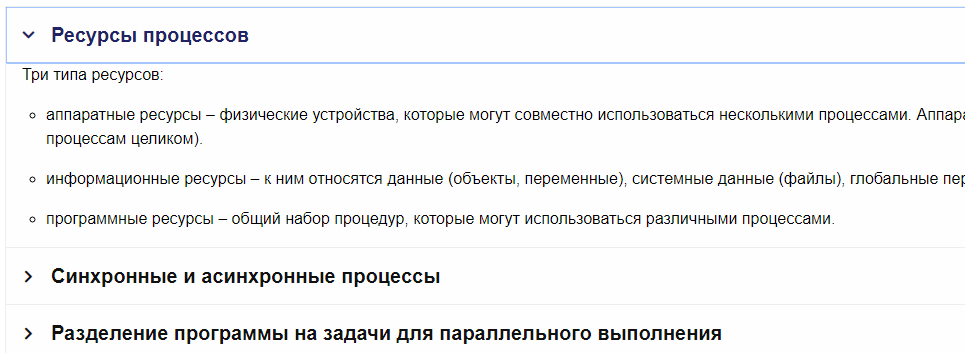
\includegraphics[width=\linewidth]{accordeon}
    \caption{Элемент \enquote{Аккордеон}}
\end{figure}

H5P элемент № 2 -- лекция, представленная \enquote{Агамотто} элементом -- весь
контент расположен последовательно друг за другом сверху вниз.

\begin{figure}[H]
    \centering
    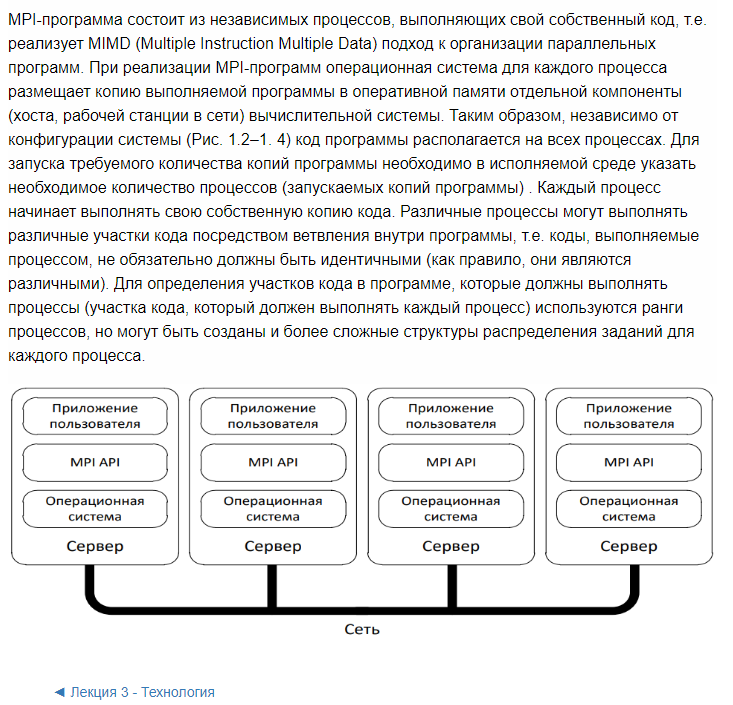
\includegraphics[width=\linewidth]{agamotto}
    \caption{Элемент \enquote{Агамотто}}
\end{figure}

\subsection*{SCORM элементы}
Добавим два упражения по алгоритмам распределенных систем. Первое упражнение:
необходимо составить алгоритм операции \enquote{Сравнить и переставить}
построчно. Строки алгоритма приведены заранее и необходимо только переставить их
местами. Реализация упражнения приведена на рисунке \ref{fig:reorder}

\begin{figure}[H]
    \centering
    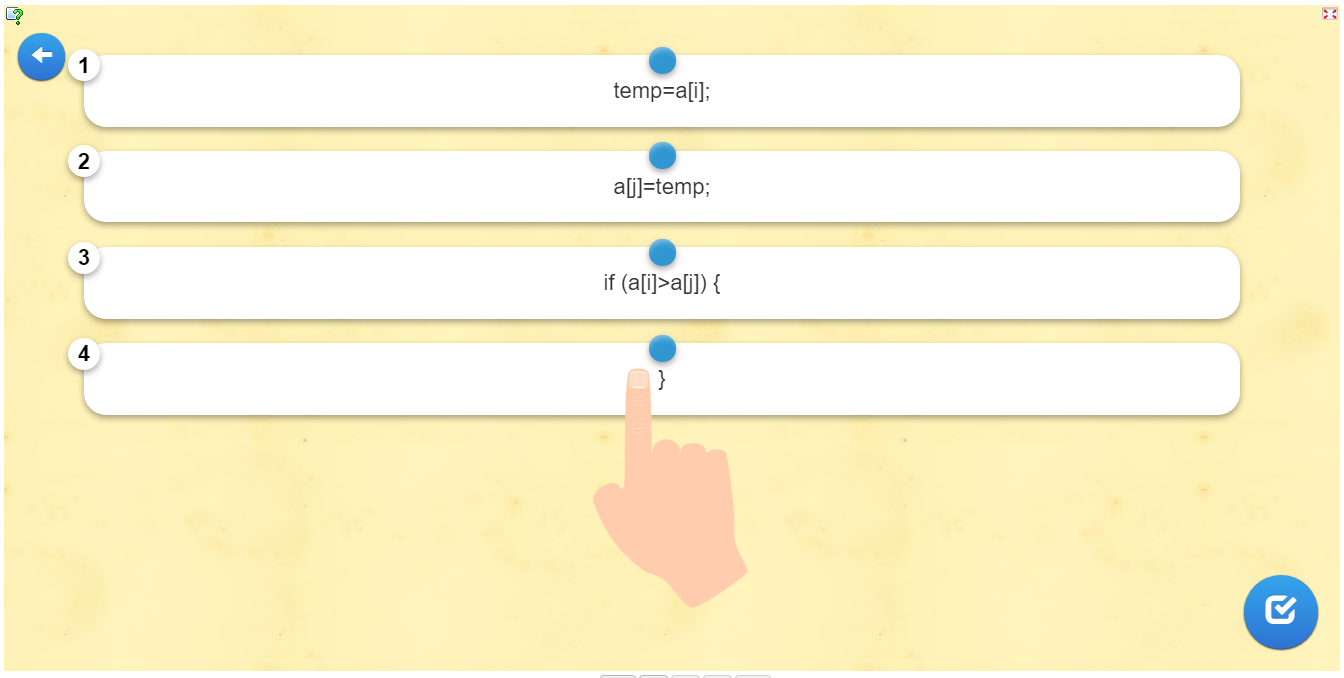
\includegraphics[width=\linewidth]{reorder}
    \caption{Упражнение на сортировку}
    \label{fig:reorder}
\end{figure}

Второе упражнение: необходимо составить правильное соответствие между функциями
MPI и их назначениями. Для этого нужно перетянуть соответствующие элементы друг
на друга:

\begin{figure}[H]
    \centering
    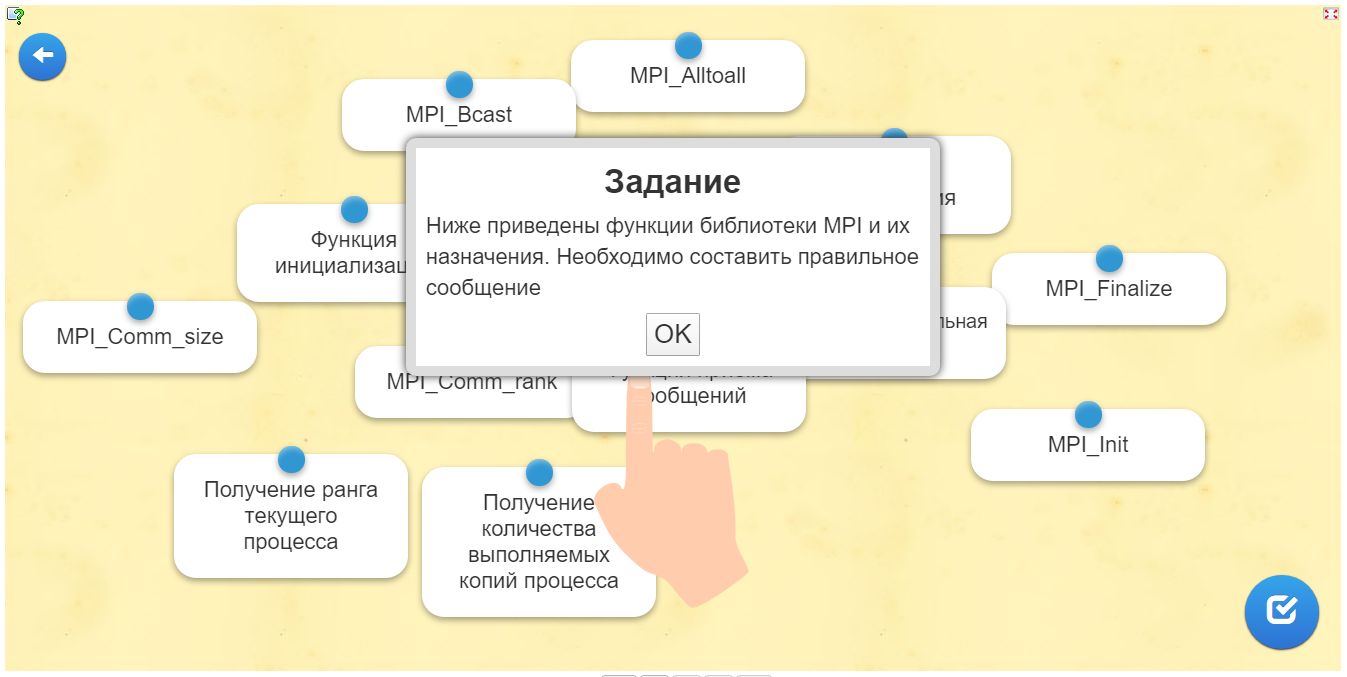
\includegraphics[width=\linewidth]{match-task}
    \caption{Условие упражнения на соответствие}
    \label{fig:match-task}
\end{figure}

\begin{figure}[H]
    \centering
    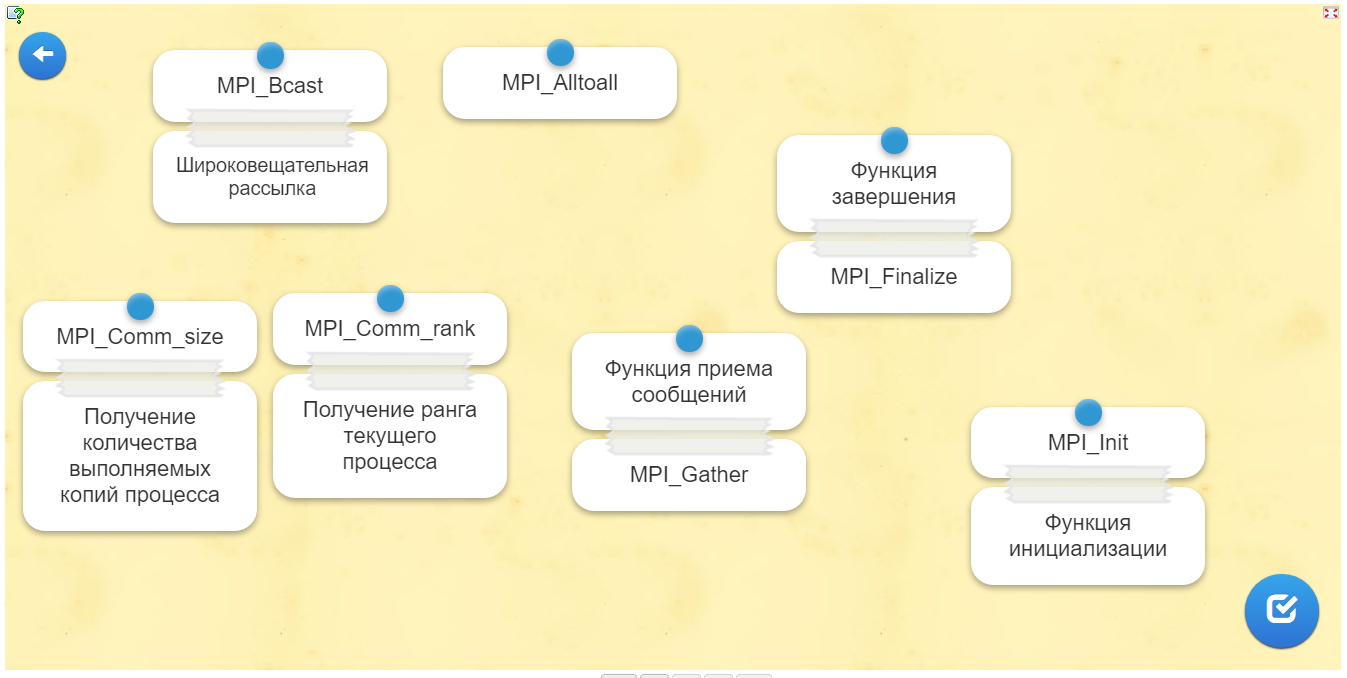
\includegraphics[width=\linewidth]{match-result}
    \caption{Ход выполнения упражнения}
    \label{fig:match-result}
\end{figure}

\end{document}